\section{Część praktyczna}
\subsection{Badanie zbiorów ``Breast cancer'' i ``Mushroom''}
Pierwszą rzeczą po zaimplementowaniu algorytmu było przetestowanie go na
zbiorach: ``Breast cancer'' oraz ``Mushroom''. Oba zbiory zostały podzielone na
dwa podzbiory: zbiór trenujący oraz zbiór testujący w relacji 3:2 w sposób
losowy.

W tabelach zostały przedstawione przykładowe wyniki uzyskane za pomocą funkcji
\textit{classification_report(actual, predicted)} z pakietu
\textit{sklearn.metrics}, gdzie \textit{actual} to rzeczywiste klasy próbek, a
\textit{predicted} to zbiór klas wyznaczonych dla tych próbek za pomocą 
algorytmu.

Na obrazkach zostały przydstawione macierze pomyłek dla zbiorów dla
przykładowych wywołań algorytmu.

\begin{table}[h!]
        \centering
        \begin{tabular}{ |p{2cm}|p{2cm}|p{2cm}|p{2cm}|p{2cm}| }
                \hline
                \multicolumn{5}{|c|}{Wyniki dla zbioru ``Breast cancer''} \\
                \hline
                 & precision & recall & f1-score & support \\
                \hline
                no-recurrence-events & 0,73 & 0,89 & 0,80 & 81 \\
                \hline
                recurrence-events & 0,44 & 0,21 & 0,28 & 34 \\
                \hline
                accuracy & - & - & 0,69 & 115 \\
                \hline
                macro avg & 0,58 & 0,55 & 0,54 & 115 \\
                \hline
                weighted avg & 0,64 & 0,69 & 0,65 & 115 \\
                \hline
        \end{tabular}
        \caption{Wyniki pomiarów dla zbioru ``Breast cancer'' przy podziale o stosunku 3:2.}
\end{table}

\begin{table}[h!]
        \centering
        \begin{tabular}{ |p{2cm}|p{2cm}|p{2cm}|p{2cm}|p{2cm}| }
                \hline
                \multicolumn{5}{|c|}{Wyniki dla zbioru ``Mushroom''} \\
                \hline
                 & precision & recall & f1-score & support \\
                \hline
                e & 1,00 & 1,00 & 1,00 & 1699 \\
                \hline
                p & 1,00 & 1,00 & 1,00 & 1551 \\
                \hline
                accuracy & - & - & 1,00 & 3250 \\
                \hline
                macro avg & 1,00 & 1,00 & 1,00 & 3250 \\
                \hline
                weighted avg & 1,00 & 1,00 & 1,00 & 3250 \\
                \hline
        \end{tabular}
        \caption{Wyniki pomiarów dla zbioru ``Mushroom'' przy podziale o stosunku 3:2.}
\end{table}



\begin{figure}[h!]
	\centering
	\begin{subfigure}[b]{0.7\linewidth}
		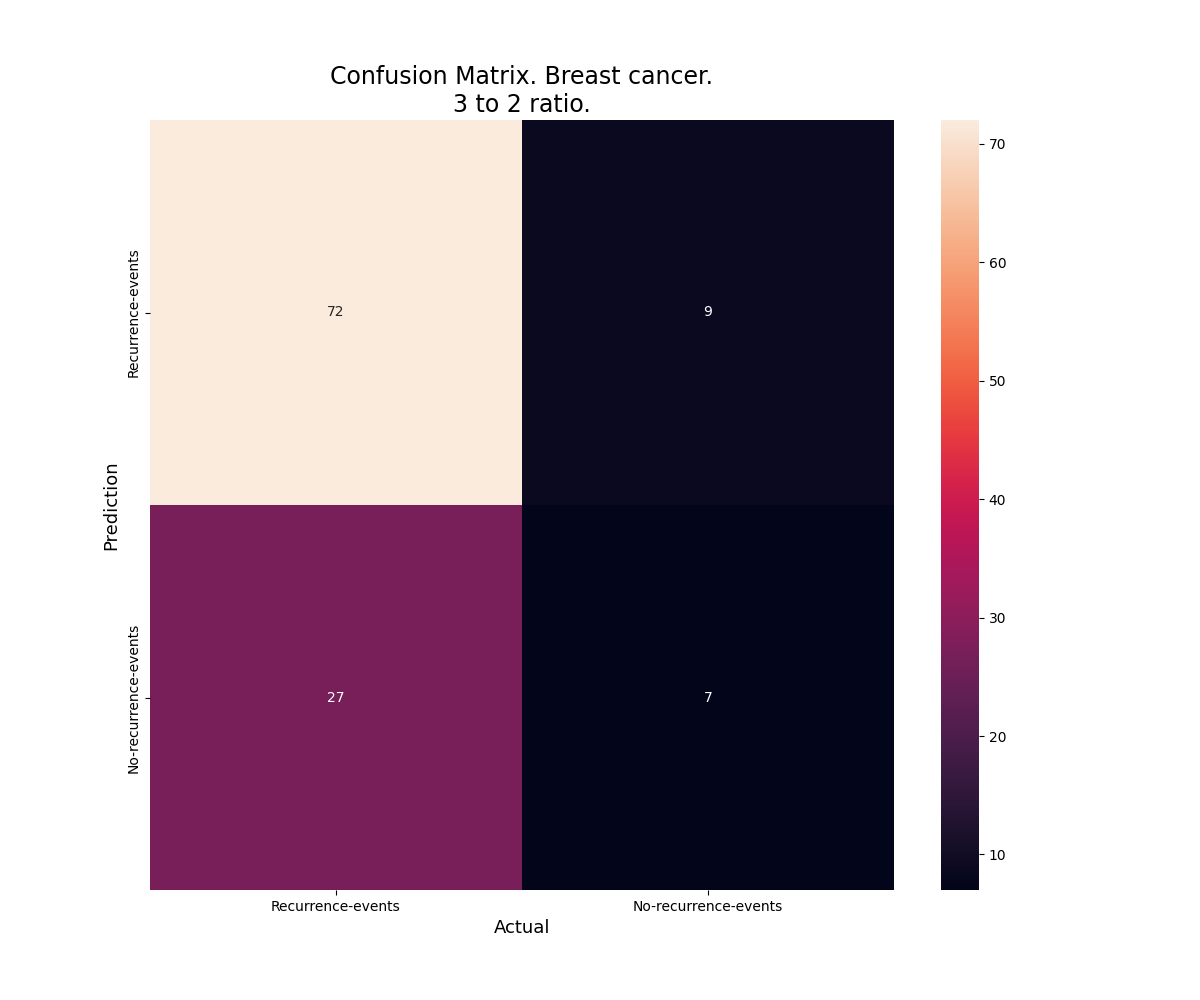
\includegraphics[width=\linewidth]{photos/bre_3_to_2_r.png}
		\caption{Macierz pomyłek dla zbioru ``Breast cancer''.}
	\end{subfigure}
	\begin{subfigure}[b]{0.7\linewidth}
		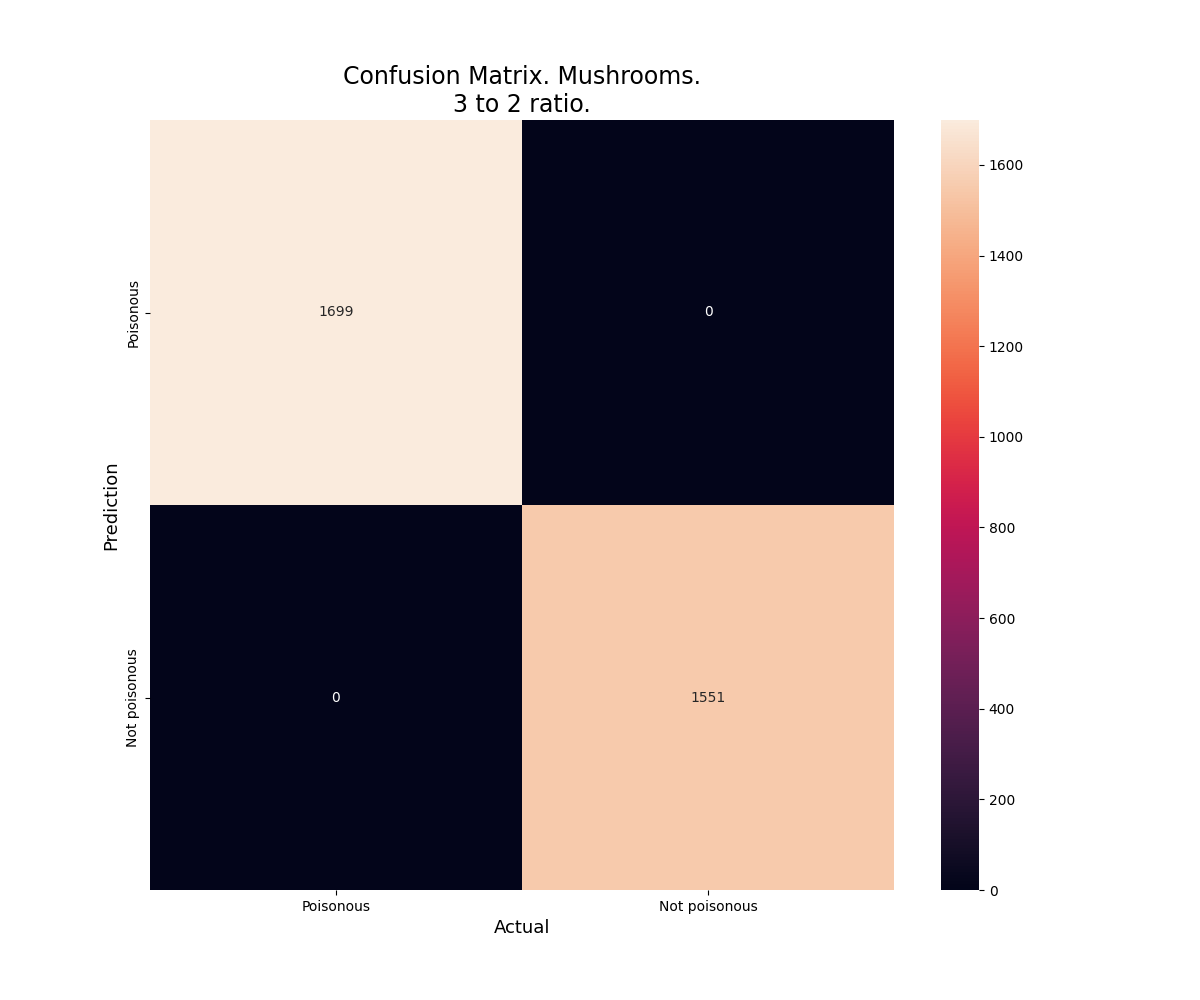
\includegraphics[width=\linewidth]{photos/mush_3_to_2_r.png}
		\caption{Macierz pomyłek dla zbioru ``Mushroom''.}
	\end{subfigure}
        \caption{Macierze pomyłek dla badanych zbiorów przy podziale o stosunku 3:2.}
\end{figure}

\clearpage

Dokładność algorytmu na zbiorze ``Breast cancer'' wyniosła 0.69, podczas gdy
dla zbioru ``Mushrooms'' wyniosła 1.00. Są to wyniki porównywalne z tymi
przedstawiony na stronie uzyskanymi dla innych algorytmów, z której zbiory
zostały pozyskane.

\subsection{Badanie zbioru ``Mushroom'' dla różych parametrów}
W dalczej części ćwiczenia zostały wykonane dodatkowe testy mające na celu
sprawdzenie, co jest przyczyną odmiennych wyników dla obu zbiorów testowanych.


Pierwszymi parametrami, które zostały sprawdzone były rozmiar zbiorów oraz
liczba atrybutów uwzględnionych w klasyfikacji.
\subsubsection{Sprawdzenie wpływu rozmiaru zbioru}
Zbiór ``Breast cancer'' zawiera 286 obiektów, podczas gdy ``Mushroom'' zawiera
ich 8124. W celu sprawdzenia, czy ma to wpływ na wyniki badań, zamiast
wykorzystywać cały zbiór ``Mushrooms'' wykorzystałem tyle obiektów, ile zawiera
zbiór ``Breast cancer''. Obiekty były wybierane w sposób losowy.


W tabeli oraz na obrazku przedstawiono rezultat badań.

\begin{table}[h!]
        \centering
        \begin{tabular}{ |p{2cm}|p{2cm}|p{2cm}|p{2cm}|p{2cm}| }
                \hline
                \multicolumn{5}{|c|}{Wyniki dla zbioru ``Mushroom''} \\
                \hline
                 & precision & recall & f1-score & support \\
                \hline
                e & 0,98 & 1,00 & 0,99 & 59 \\
                \hline
                p & 1,00 & 0,98 & 0,99 & 55 \\
                \hline
                accuracy & - & - & 0,99 & 114 \\
                \hline
                macro avg & 0,99 & 0,99 & 0,99 & 114 \\
                \hline
                weighted avg & 0,99 & 0,99 & 0,99 & 114 \\
                \hline
        \end{tabular}
        \caption{Wyniki pomiarów dla zbioru ``Mushroom'' przy podziale o stosunku 3:2.}
\end{table}

\clearpage
\begin{figure}[ht!]
	\centering
		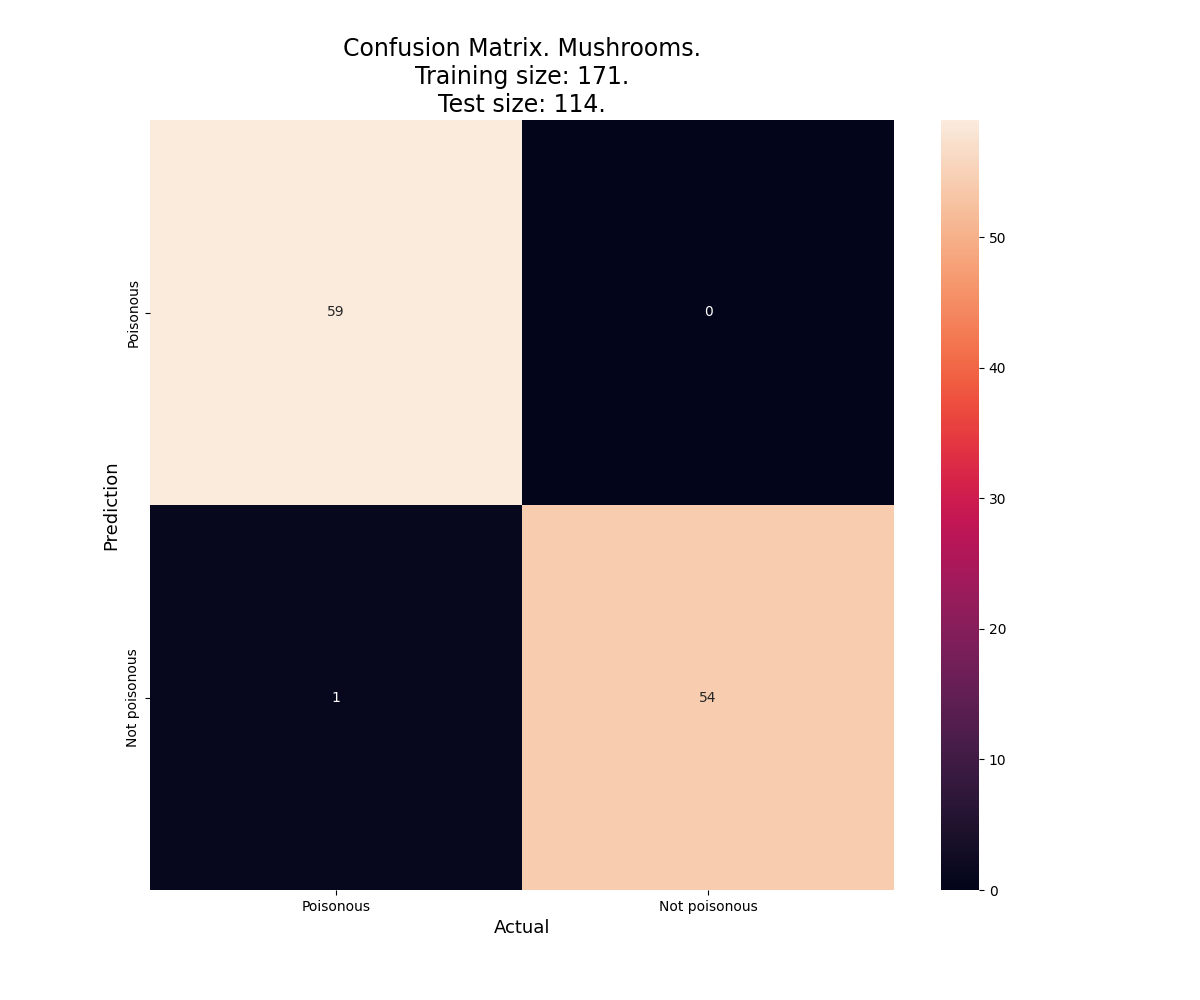
\includegraphics[width=0.7\linewidth]{photos/mush_train_size_test_size.png}
        \caption{Macierz pomyłek dla zbioru ``Mushroom'' dla rozmiaru zbioru odpowiadającemu rozmiarowi zbioru ``Breast cancer'' przy podziale o stosunku 3:2.}
\end{figure}


Z testu nie wynika, że zmniejszenie liczby próbek jest w tym przypadku źródłem
różnicy w wynikach. Algorytm ma niemal taką samą dokładność. Znacznie częściej
pojawiają się sytuacje, w których w zbiorze trenującym nie było wartości
atrybutu, który wystąpił w zbiorze testowym. Takich sytuacji nie rozwiązywałem:
wyszukiwałem inne ziarno dla generatora liczb pseudolosowych dla którego testy
przebiegały bez wystąpienia wyjątku.

Mniejszy rozmiar zbioru obiektów nie jest tutaj powodem różnic.

\subsubsection{Sprawdzenie wpływu liczby atrybutów}
Obiekty ze zbioru ``Mushroom'' są charakteryzowane przez zestaw 22 atrybutów. W
przypadku zbioru ``Breast cancer'' liczba atrybutów jest równa 9. W tym
eksperymencie, zamiast korzystać ze wszystkich atrybutów obiektów ze zbioru
``Mushroom'', wybierałem losowo 9 z nich i przeprowadzałem testy uwzględniając
tylko te wybrane.

W tabeli oraz na obrazku zostały przedstawione wyniki dla najgorszego przypadku
uzyskanego w trakcie testów.

\begin{table}[h!]
        \centering
        \begin{tabular}{ |p{2cm}|p{2cm}|p{2cm}|p{2cm}|p{2cm}| }
                \hline
                \multicolumn{5}{|c|}{Wyniki dla zbioru ``Mushroom''} \\
                \hline
                 & precision & recall & f1-score & support \\
                \hline
                e & 0,67 & 0,85 & 0,75 & 1677 \\
                \hline
                p & 0,78 & 0,56 & 0,65 & 1573 \\
                \hline
                accuracy & - & - & 0,71 & 3250 \\
                \hline
                macro avg & 0,73 & 0,71 & 0,70 & 3250 \\
                \hline
                weighted avg & 0,72 & 0,71 & 0,70 & 3250 \\
                \hline
        \end{tabular}
        \caption{Wyniki pomiarów dla zbioru ``Mushroom'' dla liczby atrybutów odpowiadającej liczbie atrybutów zbioru ``Breast cancer'' przy podziale o stosunku 3:2.}
\end{table}

\begin{figure}[h!]
	\centering
		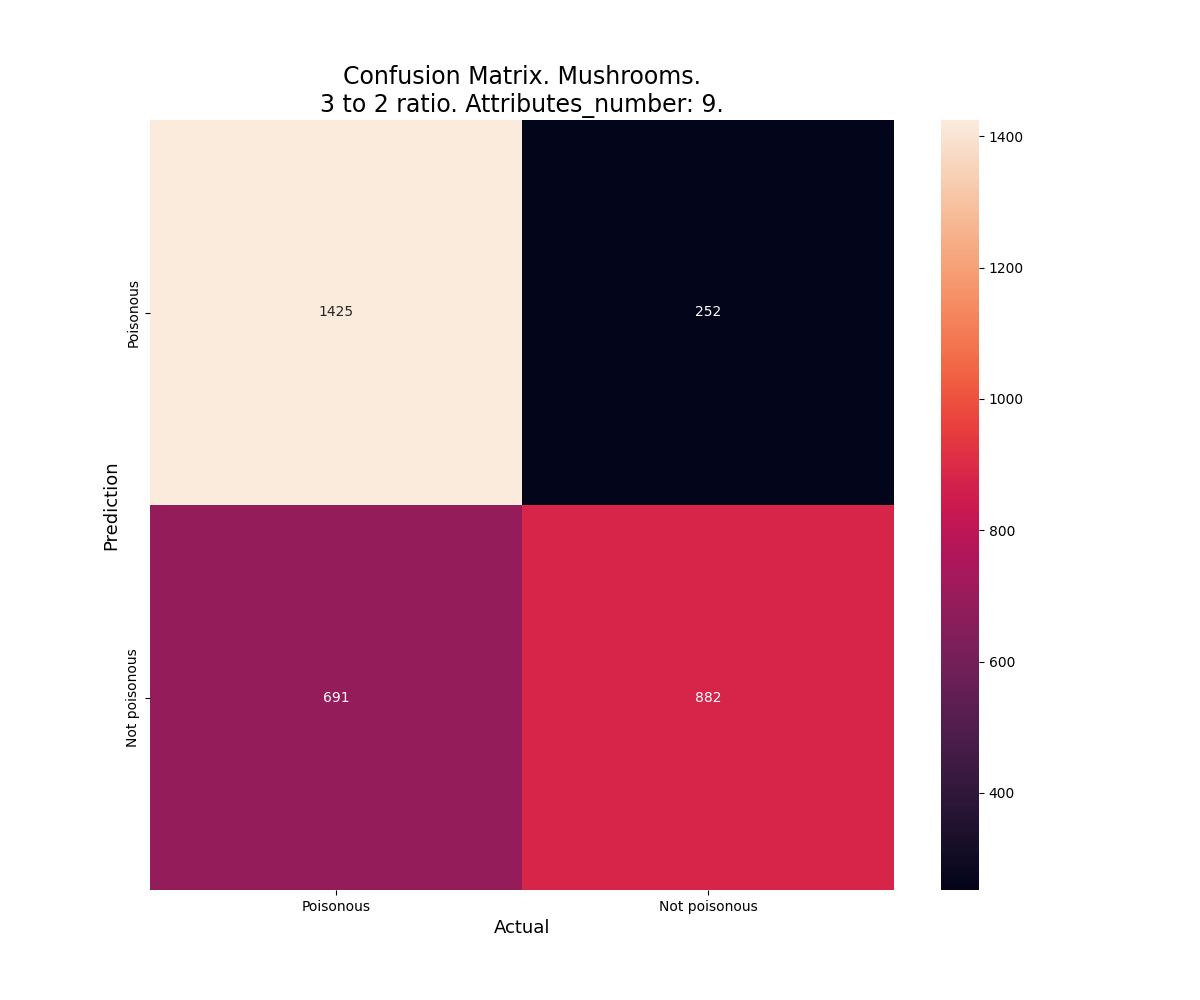
\includegraphics[width=0.7\linewidth]{photos/mush_n_attr_3_to_2_r.png}
        \caption{Macierz pomyłek dla zbioru ``Mushroom'' dla liczby atrybutów odpowiadającej liczbie atrybutów zbioru ``Breast cancer'' przy podziale o stosunku 3:2.}
\end{figure}
\clearpage

W tym eksperymencie zaobserwowałem największą do tej pory różnicę w wynikach
testów. W większości przypadków, dokładność algorytmu wynosiła ok. 100\% lub
ok. 90\%. Dla jednego przypadku jednak, uzyskałem rezultat wynoszący 71\%, co
znacząco odbiegało od dotychczasowych wyników.

Rozbieżność w wynikach może wynikać z tego, że w niektórych wywołaniach testu
do zbioru testowanego nie zostały uwzględnione atrybuty ``ważniejsze'' od
pozostałych. Mniejsza liczba atrybutów zmniejsza możliwość wyboru najlepiej
dzielącego zbiór atrybutu w danej gałęzi drzewa.

\subsubsection{Zastosowanie rozmiaru zbiorów oraz liczby atrybutów takiej, jaka
jest w zbiorze ``Breast cancer''}
W tym eksperymencie niejako zostały połączone dwa podejścia wykonane w
powyższych punktach.

W tabeli i na obrazku przedstawiono rezultaty jednego z testów.

\begin{table}[h!]
        \centering
        \begin{tabular}{ |p{2cm}|p{2cm}|p{2cm}|p{2cm}|p{2cm}| }
                \hline
                \multicolumn{5}{|c|}{Wyniki dla zbioru ``Mushroom''} \\
                \hline
                 & precision & recall & f1-score & support \\
                \hline
                e & 1,00 & 1,00 & 1,00 & 52 \\
                \hline
                p & 1,00 & 1,00 & 1,00 & 62 \\
                \hline
                accuracy & - & - & 1,00 & 114 \\
                \hline
                macro avg & 1,00 & 1,00 & 1,00 & 114 \\
                \hline
                weighted avg & 1,00 & 1,00 & 1,00 & 114 \\
                \hline
        \end{tabular}
        \caption{Wyniki pomiarów dla zbioru ``Mushroom'' dla liczby atrybutów oraz rozmiaru zbioru odpowiadającym liczbie atrybutów i romiarowi zbioru ``Breast cancer'' przy podziale o stosunku 3:2.}
\end{table}

\clearpage
\begin{figure}[h!]
	\centering
		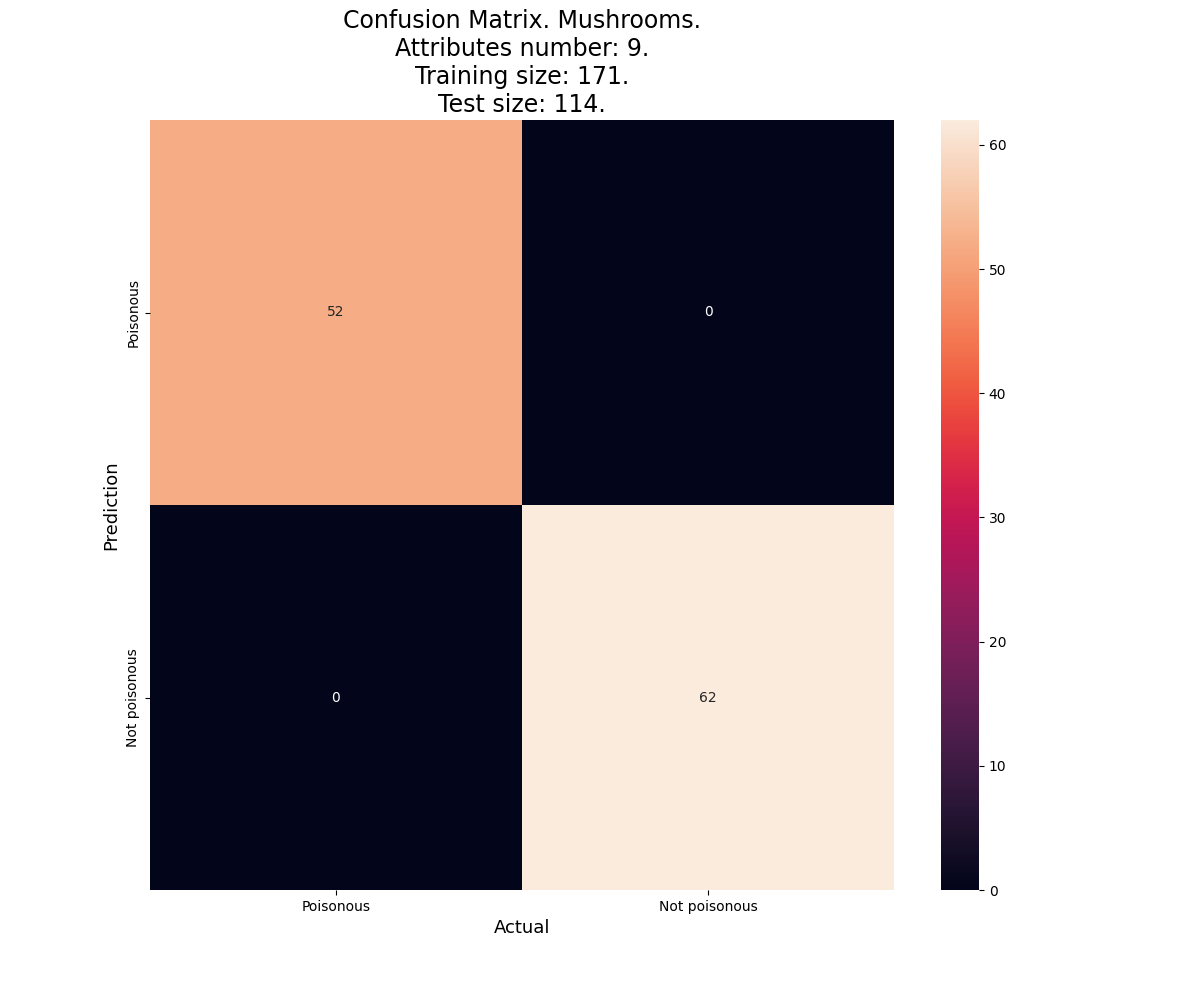
\includegraphics[width=0.7\linewidth]{photos/mush_n_attr_train_size_test_size.png}
        \caption{Macierz pomyłek dla zbioru ``Mushroom'' dla liczby atrybutów oraz rozmiaru zbioru odpowiadającym liczbie atrybutów i romiarowi zbioru ``Breast cancer'' przy podziale o stosunku 3:2.}
\end{figure}

Nie zaobserwowano pogorszenia się wyników względem pierwotnego wyniku.

\subsection{Wpływ poszczególnych atrybutów w zbiorze na wyniki predykcji}
Wiedząc, że atrybuty mogą mieć wpływ na wyniki testów chciałem sprawdzić, jaki
wpływ na klasę obiektu ma każdy atrybut. Zostało to przetestowane z użyciem
klas \textit{RandomForestRegressor} \textit{RandomForestClassifier} z biblioteki
\textit{sklearn.ensemble}. Wartości atrybutów zostały zamapowane na liczby.

Na obazka zostały przedstawione ``ważności'' poszczególnych atrybutów dla
określonych zbiorów.

\begin{figure}[h!]
	\centering
	\begin{subfigure}[b]{0.6\linewidth}
		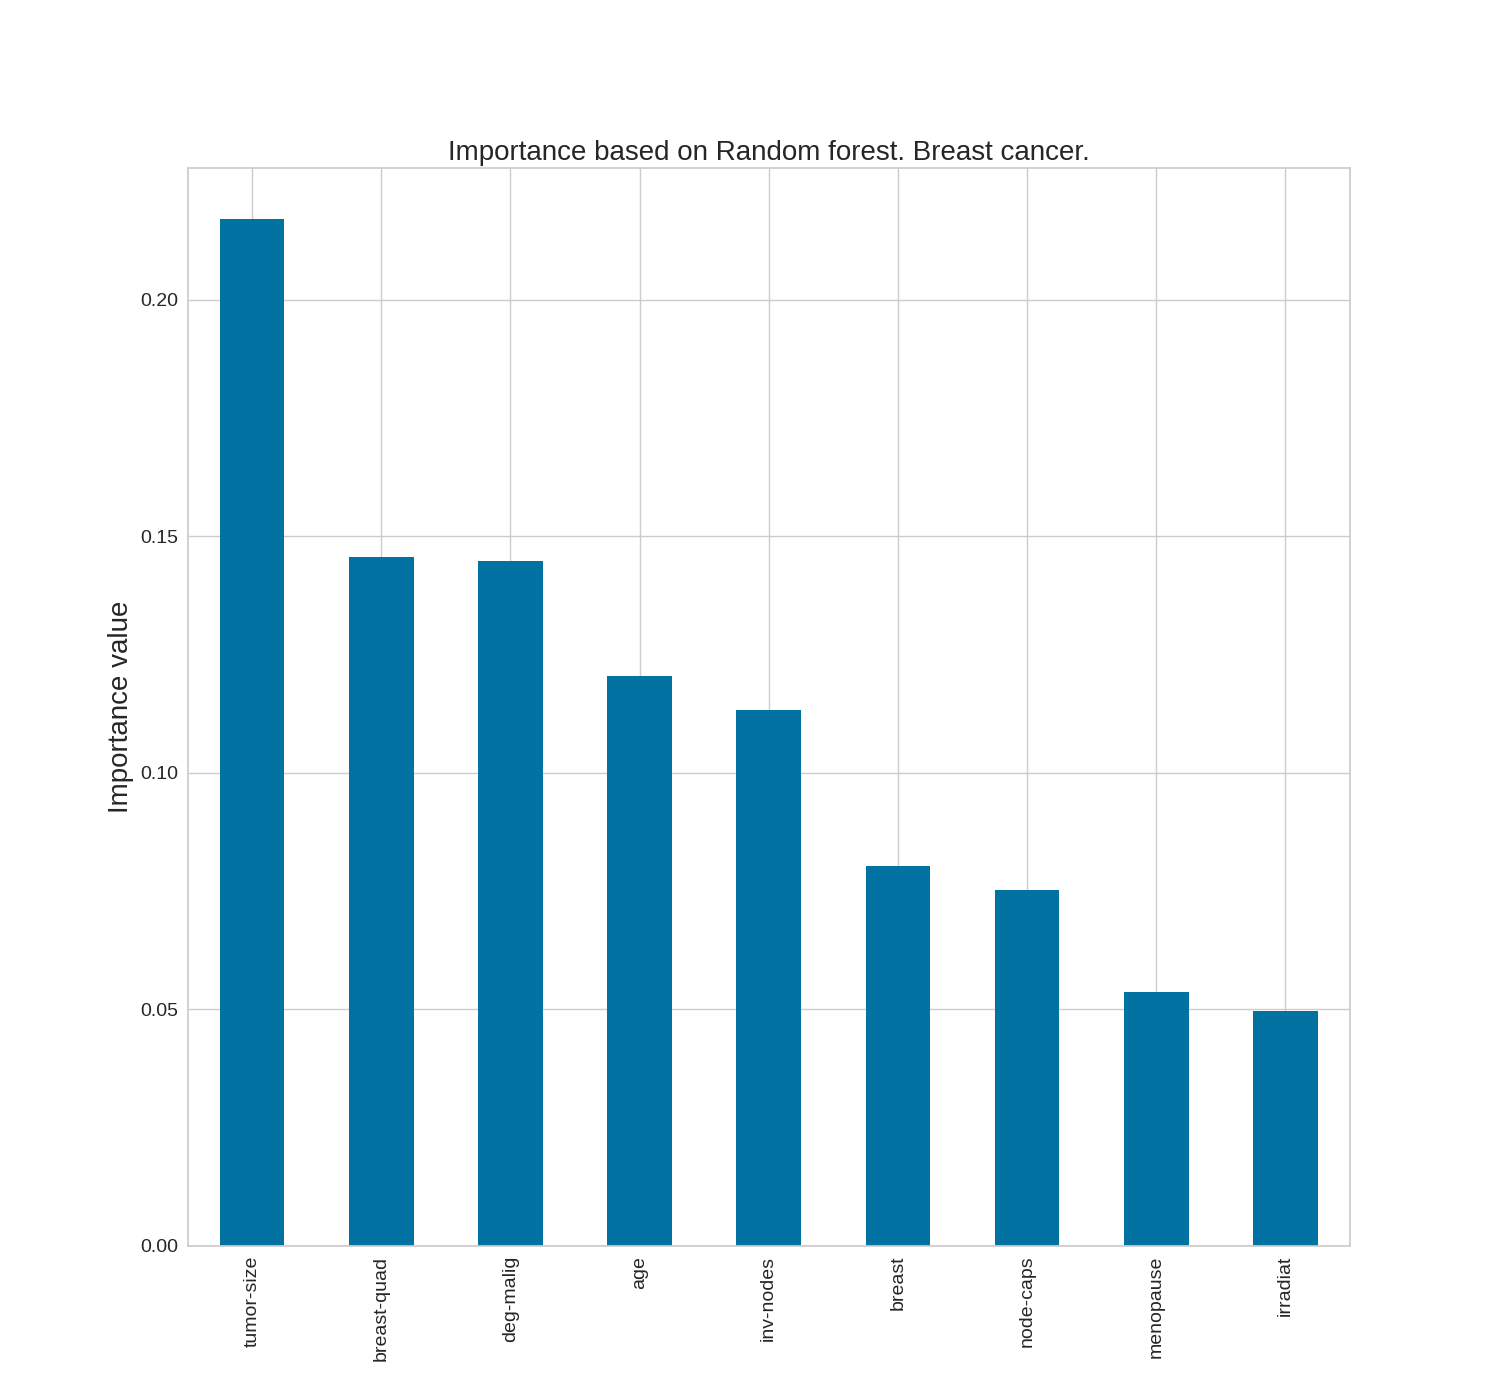
\includegraphics[width=\linewidth]{photos/importances_bre.png}
		\caption{``Breast cancer''}
	\end{subfigure}
	\begin{subfigure}[b]{0.6\linewidth}
		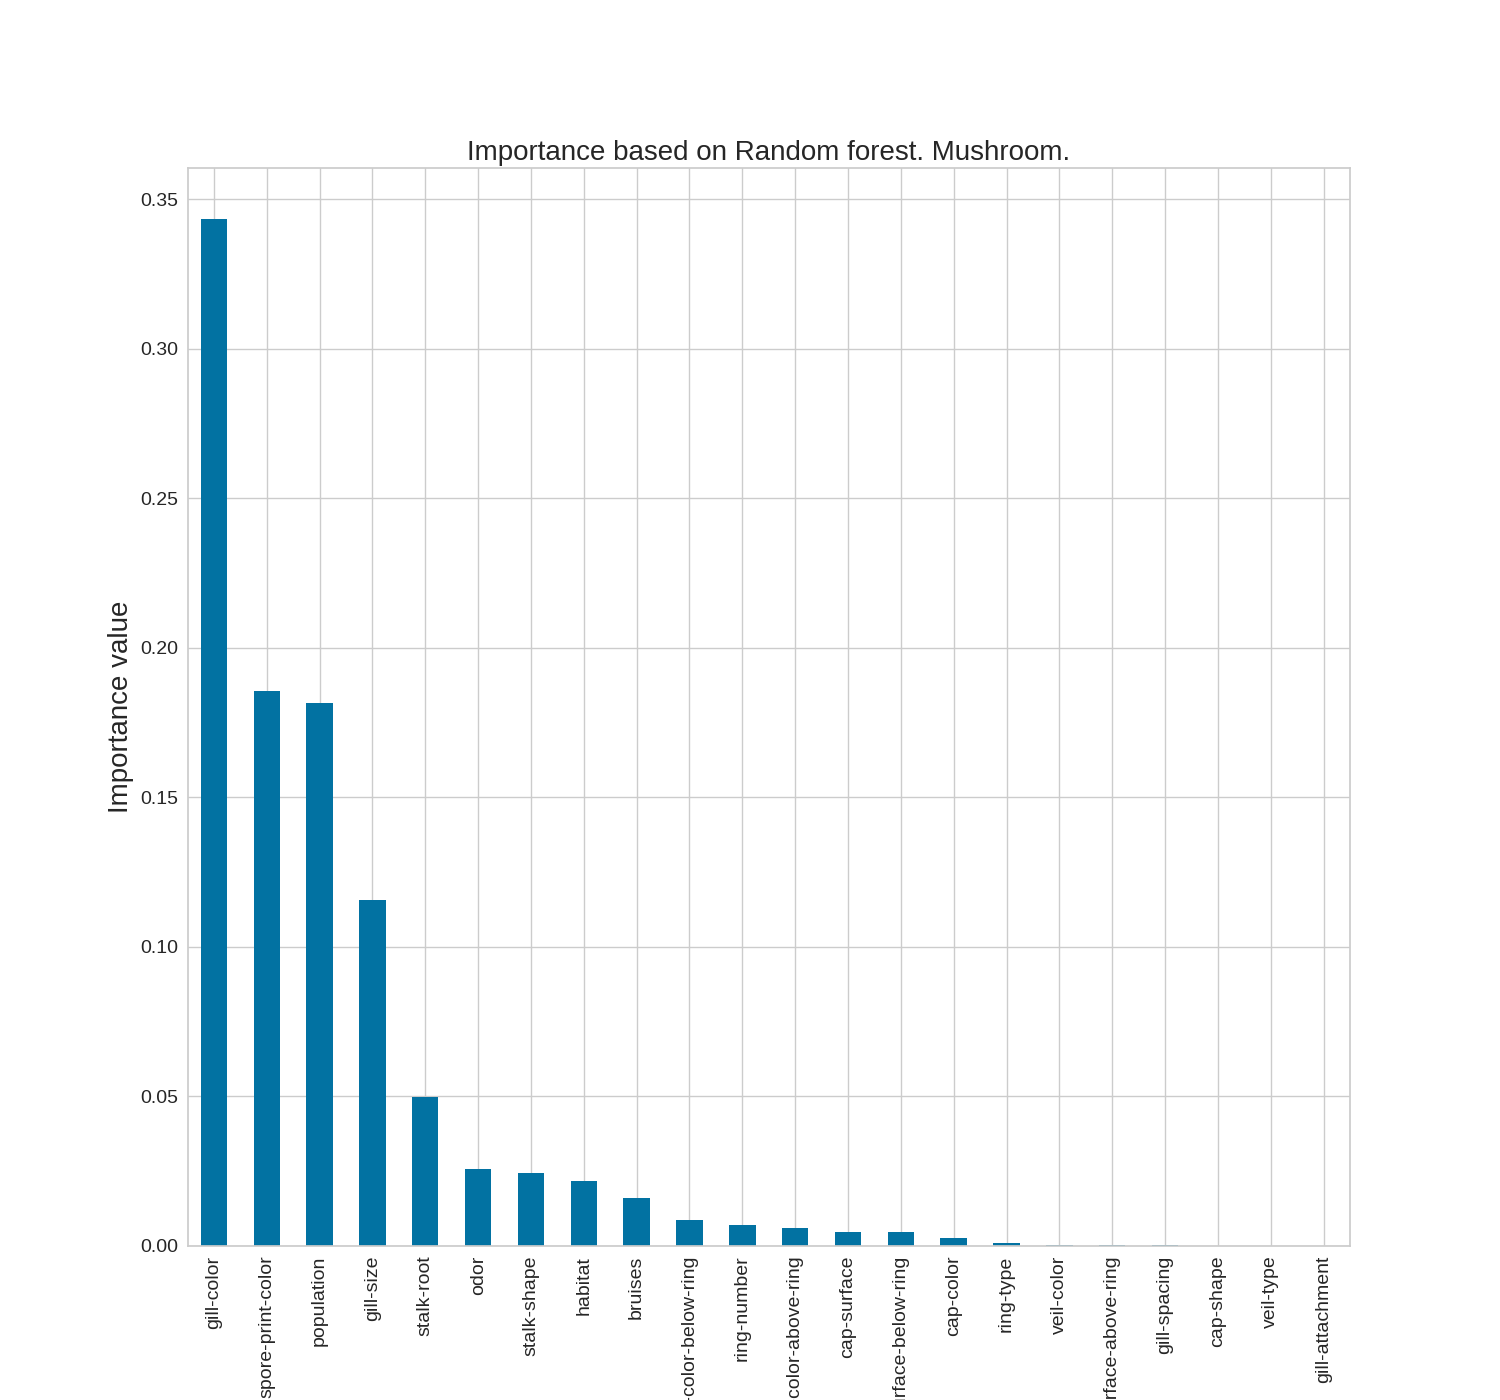
\includegraphics[width=\linewidth]{photos/importances_mush.png}
		\caption{``Mushroom''}
	\end{subfigure}
        \caption{Wykresy przedstawiające ``ważności'' poszczególnych atrybutów przy klasyfikacji.}
\end{figure}
\clearpage

W zbiorze ``Mushroom'' najbardziej znaczącym atrybutem jest \textit{gill-color}.
Jego ważność została oceniona na 0.35. W zbiorze ``Mushrooms'' duża część
atrybutów ma znikome znaczenie przy tworzeniu drzewa decyzyjnego. Może to
sugerować, że decyzja o tym, do jakiej klasy należy dany obiekt jest podejmowana
znacznie wcześniej, czyli i głebokość drzewa decyzyjnego jest niższa. Świadczy
to o tym, że istnieją atrybuty które bardzo dobrze rozdzielają zbiór obiektów
na maksymalnie różne podzbiory za pomocą wyliczania entropii zbiorów.

Dla zbioru ``Mushroom'' 5 atrybutów ma wpływ większy niż 0.05, podczas gdy dla
zbioru ``Breast cancer'' wszystkie atrybuty miały znaczenie o wartości
równej co najmniej 0.05.
